% !TEX root = ../../../I4PRJ, Grp3 - Rapport.tex
\section{Applikationslaget}
Applikationslaget er det lag af software i det samlede distribuerede system, som installeres eller afvikles hos brugeren. Applikationslaget er designet til at være platformuafhængigt, jf. systemets arkitektur. Lagets model- og præsentationslag er designet til at være portabelt, hvorimod view-laget er platformspecifikt og designes seperat for hver platform. 

Det overordnede design i applikationslaget illustreres ved sekvensdiagrammet i figur~\ref{fig:application_sd}. Her fremgår kommunikationsmønsteret mellem model-, view- og presenter-klasserne i applikationslagets design.

\begin{figure}
	\centering
	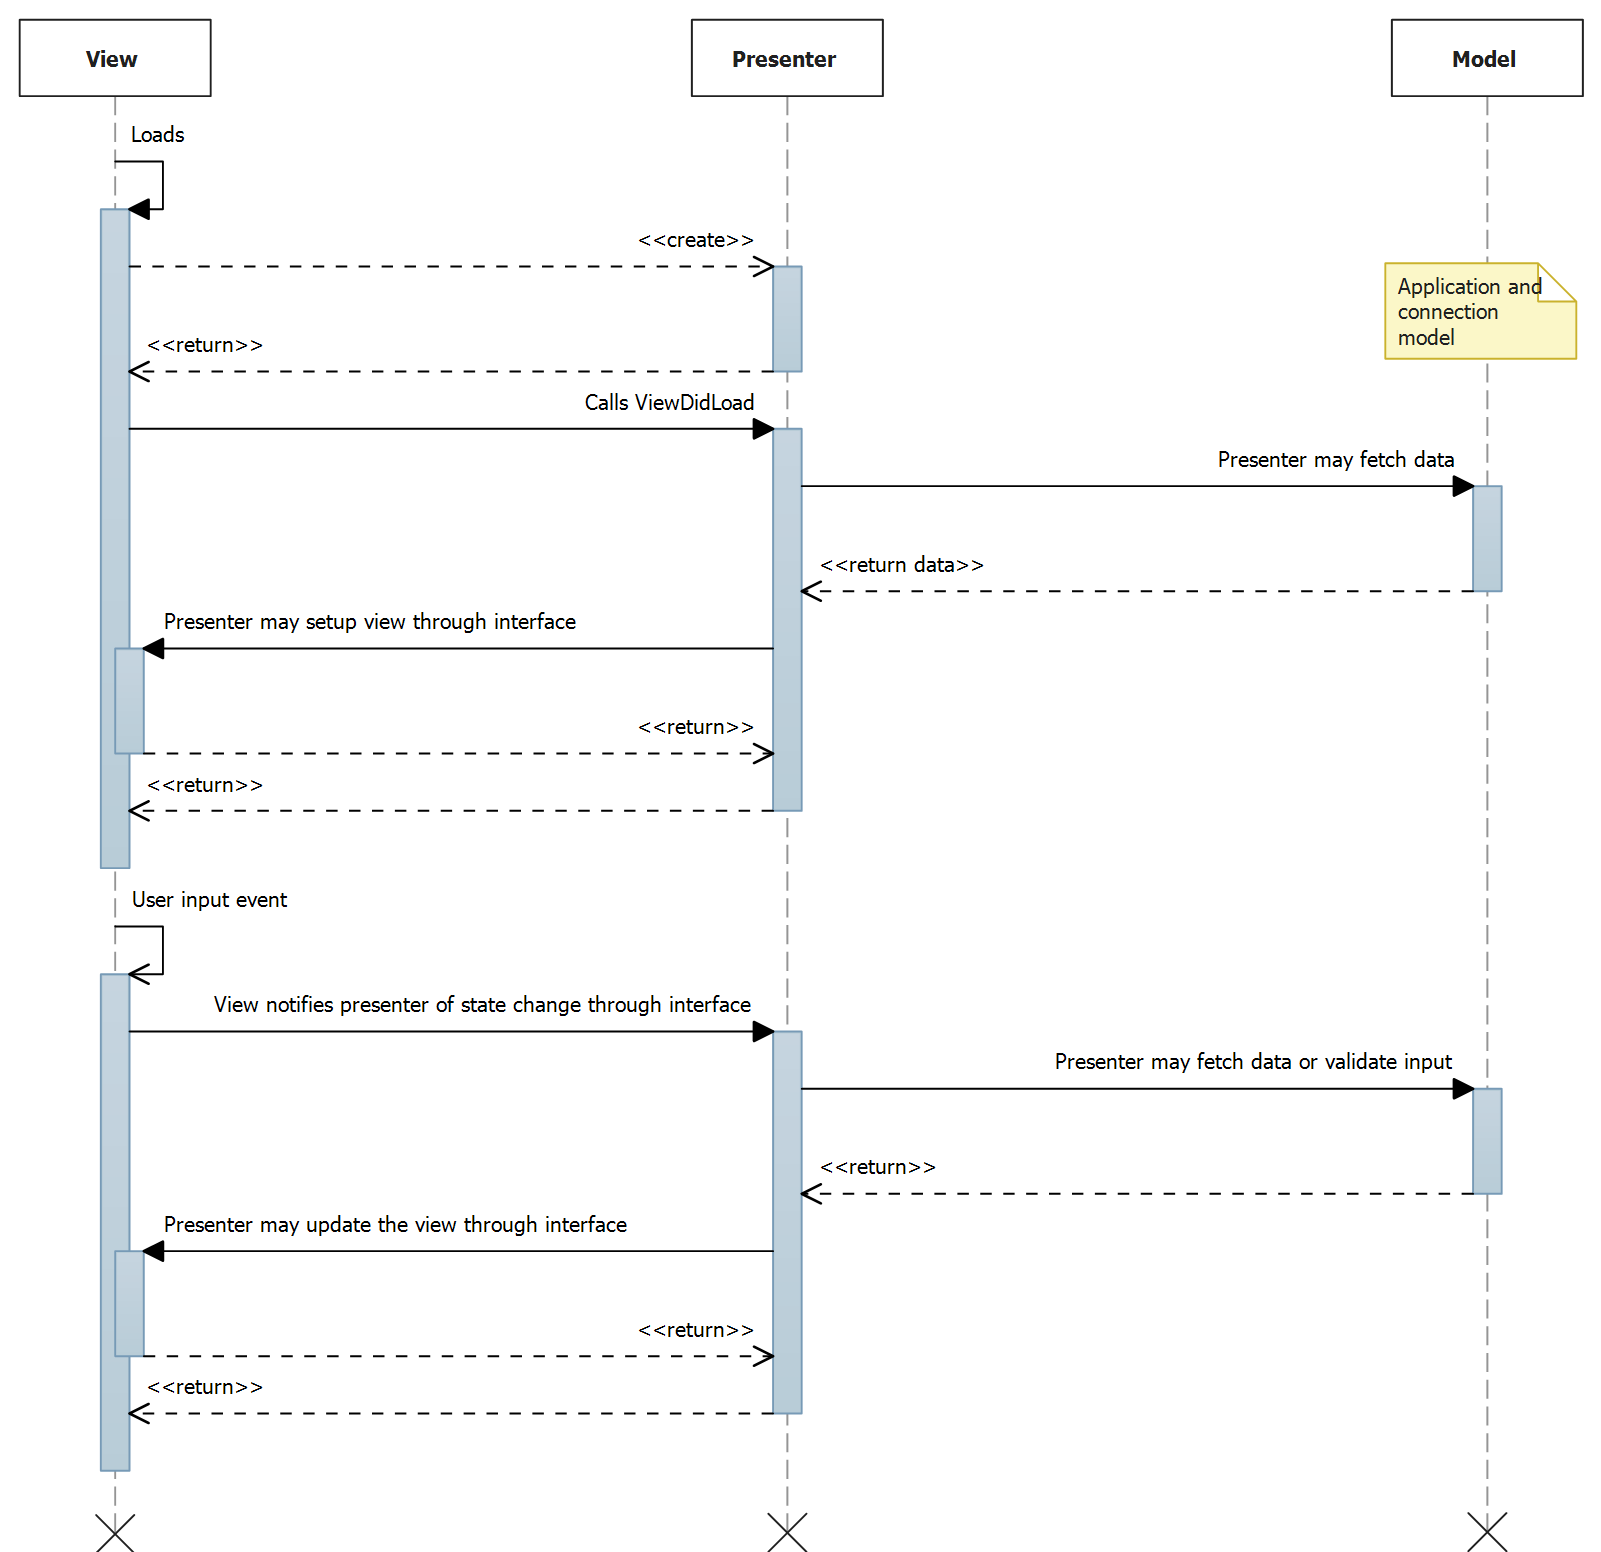
\includegraphics[width=1.0\linewidth]{figs/design/application_sd}
	\caption{Kommunikation i applikationslaget}
	\label{fig:application_sd}
\end{figure}

Som følge systemets multi-lag arkitektur kunne applikationslaget samt de platform-specifikke view-implementeringer
designes, uafhængigt af hinanden, så længe protokolbestemmende interfaces blev specificeret undervejs i processen. Interfaces for både presenters og views, er defineret ud fra de user stories, der har krævet deres design.

Præsentationslaget består af interfaces til presenters og views, samt konkrete presenters-klasser. View interfaces specificeres af de tilhørende presenter-klasser, og definerer presenter-klassens interaktion med view'et. På figur~\ref{fig:application_isignupview} ses klassediagrammet for ISignUpView-interfacet.

\begin{figure}
\centering
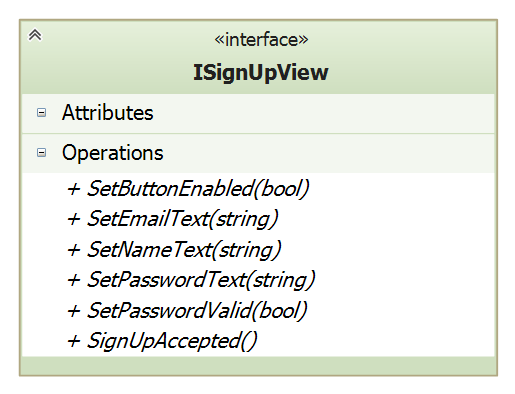
\includegraphics[width=0.35\linewidth]{figs/design/application_isignupview}
\caption{ISignUpView}
\label{fig:application_isignupview}
\end{figure}

Det konkrete signup view i hver platformspecifikke applikation implementerer view-interfacet og instantiere den tilhørende controller, hvis interface- og klassedesign ses på figur~\ref{fig:application_isignupviewcontroller}.

\begin{figure}
\centering
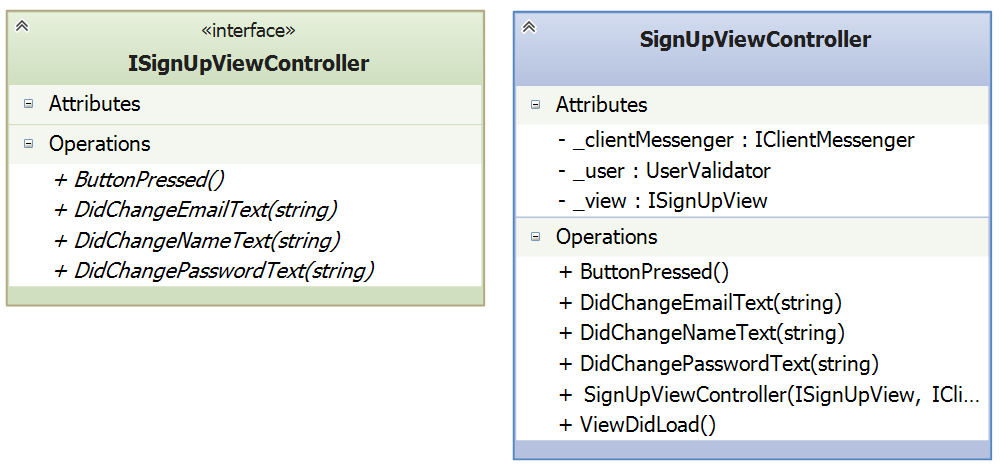
\includegraphics[width=0.7\linewidth]{figs/design/application_signupviewcontrollerandinterface}
\caption{ISignUpViewController og SignUpViewController}
\label{fig:application_isignupviewcontroller}
\end{figure}
Figur~\ref{fig:application_isignupviewcontroller} viser også, at den konkrete klasse indeholder flere metoder og attributter, som binder den konkrete klasse sammen med modellen. Modellen i applikationslaget består delvist af valideringslogik og klasser til kommunikation med resten af systemet. Det er attributter som \_clientMessenger, som er klienten, der kommunikerer med serveren og \_user af typen UserValidater, der validere om brugerinformationen er gyldig.

Den user story der omhandler visning af målinger, har ført til designet af følgende presenter-klasse.

\begin{figure}
\centering
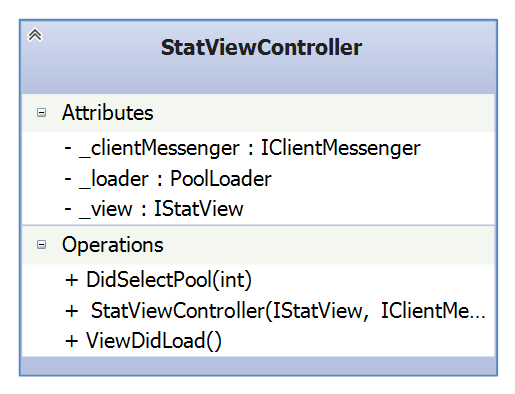
\includegraphics[width=0.35\linewidth]{figs/design/application_statviewcontroller}
\caption{StatViewController konkret klasse}
\label{fig:application_statviewcontroller}
\end{figure}

For yderligere forklaring se dokumentation afsnit Applikationslaget under Design.

\subsection{Windows GUI}
I Windows applikationen designes view-klasser, der implementerer view-interfacet defineret i præsentationslaget.
Designet af Windows GUI er lavet således, at codebehind filerne implementerer hver sit view-interfacet fra præsentationslaget. Codebehind agerer dermed som en bro, i mellem Smartpools præsentationslag, og WPF view-lag.

I klasse diagrammet nedenfor, ses Windows designet, af WinCreateUserView der implementerer ISignUpView fra applikationslaget og har en SignUpViewController.
\begin{figure}
\centering
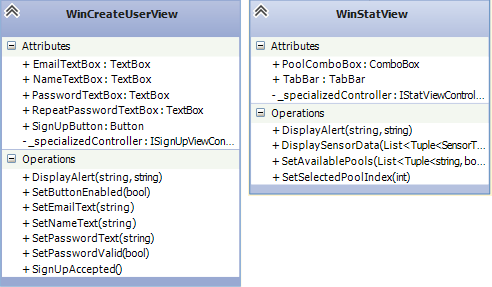
\includegraphics[width=0.7\linewidth]{figs/design/wincreateuserandwinstatviewview}
\caption{WinCreateUserView og WinStatView}
\label{fig:wincreateuserandwinstatviewview}
\end{figure}

Ligeledes er view klassen for WinStatView designet.
Klassen ses på figur~\ref{wincreateuserandwinstatviewview}.

For yderligere forklaring se dokumentation afsnit Applikationslaget under Design.

<<<<<<< HEAD
\subsection{iOS}
I iOS applikationen designes view-klasser, der implementerer view-interfacet defineret i præsentationslaget. Det dominante user interface framework på iOS kaldes UIKit, og det er bygget op omkring en model-view-controller arkitektur. I UIKit har hvert view en tilhørende controller-klasse. I iOS designet tages der højde for dette, ved at bruge controller-klassen som en bro, i mellem Smartpools præsentationslag, og UIKits view-lag. Designet er derfor lavet således, at controller-klasserne på iOS implementerer view-interfacet fra præsentationslaget.

\subsubsection{SignUpViewBridge}
SignUpViewBridge-klassen implementerer ISignUpView interfacet. Klassen indeholder en række UIKit user interface elementer, som passer sammen med interfacet. Da dette view omhandler brugeroprettelse, er klassen designet til at indeholde en række tekstfelter, og en knap til at fuldende brugeroprettelsen. Denne klasse er designet til at nedarve fra UIKit klassen UIViewController, da de user interface elementer der indgår i designet, forventes at være statiske.

\begin{figure}
	\centering
	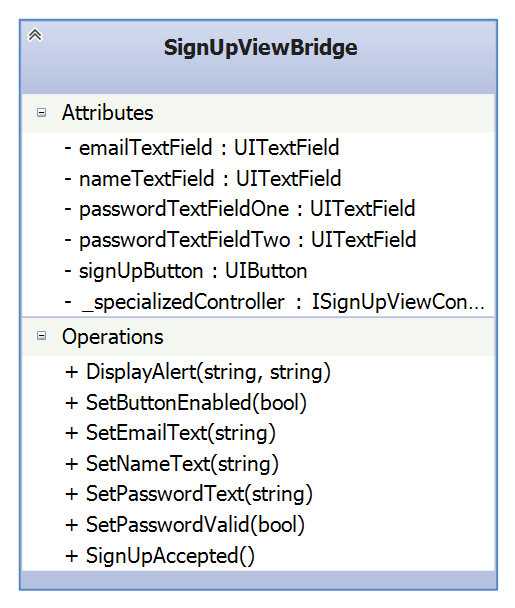
\includegraphics[width=0.3\linewidth]{figs/design/ios_signupviewbridge}
	\caption{SignUpViewBridge}
	\label{fig:ios_signupviewbridge}
\end{figure}

\subsubsection{StatViewBridge}
StatViewBridge-klassen implementerer IStatView interfacet. Dette view bør kunne håndtere dynamisk indlæsning og visning af måledata i følge de user stories, der er tilknyttet interfacet. Af denne grund nedarver StatViewBridge fra UITableViewController, der kan opsættes til at præsentere en dynamisk liste. StatViewBridge indeholder en UIBarButtonItem, der kan bruges til at skifte imellem pools i systemet.

\begin{figure}
	\centering
	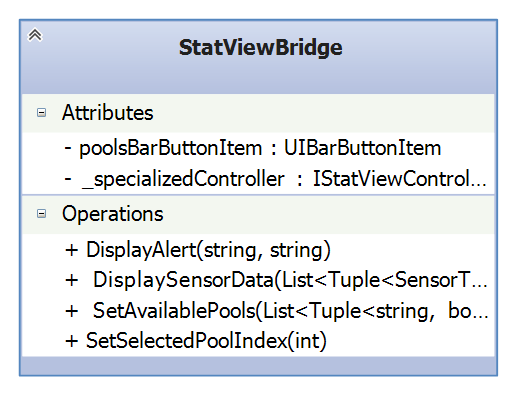
\includegraphics[width=0.3\linewidth]{figs/design/ios_statviewbridge}
	\caption{StatViewBridge}
	\label{fig:ios_statviewbridge}
\end{figure}
For yderligere forklaring se dokumentation afsnit Applikationslaget under Design.
% !TEX root = ../../../I4PRJ, Grp3 - Rapport.tex
\chapter{Grafisk Design}
I dette afsnit beskrives det grafiske design af brugergrænsefladen. Det grafiske design skal afspejle de respektive views funktionalitet. Først udarbejdes et konceptuelt design. GUI views designes ved at analyserer og diskuterer user stories for systemet. Resultatet af analysen er et håndtegnet design med tilhørende noter fra diskussionerne. Analyseresultatet dannede grundstenene for GUI folkenes arbejde. Designet blev dermed ensartet for de forskellige platforme. Det fælles udarbejdede design har mindsket en muligt senere kommende bureaukratisk proces, da alle udviklere ved at målet er nået, når GUI svarer til design. 

\section{Konceptuel Design}
Først udarbejdes et konceptuelt design. Det konceptuelle design udarbejdes ved analyse og diskussion af user stories, som eksempel er user story omhandlende login behandlet og kan ses på figuren nedenfor:

\begin{figure}
	\centering
	\includegraphics[width=\linewidth]{figs/design/konceptuel_design_loginview}
	\caption{Domænemodel for systemet}
	\label{fig:domainmodel}
\end{figure}

De forskellige platformes GUI minder i så høj grad om hinanden, at hvert view og hvilke user stories de implementerer kun vil blive beskrevet for en platform. 
\subsection{Farvepalet}
For at opfylde kvalitetskravet, at applikationer skal være visuelt ensartede, er der under det visuelle design lavet en Smartpool farvepalet.
\begin{table}[]
\centering
\begin{tabular}{ll}
SpBlack          & \cellcolor[HTML]{0A0A0A}{\color[HTML]{FFFFFF} \#FF0A0A0A} \\
SpDarkGrey       & \cellcolor[HTML]{1F1F1F}{\color[HTML]{FFFFFF} \#FF1F1F1F} \\
SpGrey           & \cellcolor[HTML]{575757}{\color[HTML]{FFFFFF} \#FF575757} \\
SpLightGrey      & \cellcolor[HTML]{ABABAC}\#FFABABAC                        \\
SpOrange         & \cellcolor[HTML]{FDA029}\#FFFDA029                        \\
SpRed            & \cellcolor[HTML]{FF584D}\#FFFF584D                        \\
SpLightBlue      & \cellcolor[HTML]{49BAE1}\#FF49BAE1                        \\
SpBlue           & \cellcolor[HTML]{0354A5}\#FF0354A5                        \\
SpWhite          & \cellcolor[HTML]{FFFFFF}\#FFFFFFFF                        \\
SpBackgroundGray & \cellcolor[HTML]{2E2E2E}{\color[HTML]{FFFFFF} \#FF2e2e2e} \\
SpAccentGray     & \cellcolor[HTML]{3E3E3E}{\color[HTML]{FFFFFF} \#FF3e3e3e}
\end{tabular}
\caption{Farvepalet}
\label{table:farvepalet}
\end{table}
